\documentclass[article,oneside]{memoir}
\usepackage[utf8]{inputenc}

\usepackage{amsmath}
\usepackage{amssymb}
\usepackage{indentfirst}
\usepackage{pythonhighlight}
\usepackage{tikz}
\usepackage{multirow}
\usepackage{float}
\usepackage[a4paper, total={7in, 9in}]{geometry}

\title{GLCM Vectorizing through NumPy}
\date{2020\\ October}
\author{John Chang\\ Nanyang Technological University}

\begin{document}
\maketitle
\newpage

\chapter{Introduction}

This is written on the assumption that the reader understands GLCM.

As we understand, the Gray Level Co-occurrence Matrix is a separately generated matrix to calculate statistics such as \textbf{Contrast, Correlation and Entropy}.

However, from a programming perspective, it's computationally expensive and redundant.

In this, we'll discuss how to vectorize the operations for \textbf{Contrast and Correlation}, then discuss issues with vectorizing \textbf{Entropy}.

\section{Preamble}

The main issue with creating a GLCM is due to NumPy vectorizing not being able to work around it.

Consider the following:

\begin{python}
a = [1,2,1,4,5]
b = [1,3,1,5,5]

c = np.vstack([a,b])

print(np.unique(c, return_counts=True, axis=1))
\end{python}

Returns the following:

\begin{verbatim}
(array([[1, 2, 4, 5],
        [1, 3, 5, 5]]),
 array([2, 1, 1, 1], dtype=int64))
\end{verbatim}

This is a suitably fast enough operation if we needed the \verb+counts+. However, \verb+np.unique+ is a large bottleneck on larger scale data.

Can we calculate all 3 statistics \textit{(Contrast, Correlation and Entropy)} without calling \verb+np.unique+?

\subsection{Vanilla Conventions}

These conventions are used in the GLCM context, whereever it's generated.

$i, j$ Represents the labels on the 2 sides of the GLCM.

$n_{i, j}$ Represents the GLCM count for index $i, j$

$$\sum_{i=i_0,j=j_0}^{i=i,j=j}f(i, j, n_{i,j})$$

Means to loop through all cells, $i_0$ and $j_0$ can be arbitrarily defined. However it is paramount that it loops through all cells once.

$f(i, j, n_{i,j})$ is defined as the function that will occur on every $i, j$ pair before summation.

\subsection{Offset Arrays}

GLCM generates itself by looking at a neighbour at a fixed offset. Instead of creating the GLCM right away, we can generate 2 arrays.

\begin{enumerate}
\item{Original Array $a$}
\item{Target Array $b$}
\end{enumerate}

$a, b$ Represents the original and target matrices.

\textit{Doesn't matter which is called the original or target.}

\subsection{Making Pairs}

One important aspect of this is that we make 2 matrices with a single one by overlaying one with another.

The shift is manually defined, in this we will shift diagonally by 1.

\begin{figure}[H]
\centering
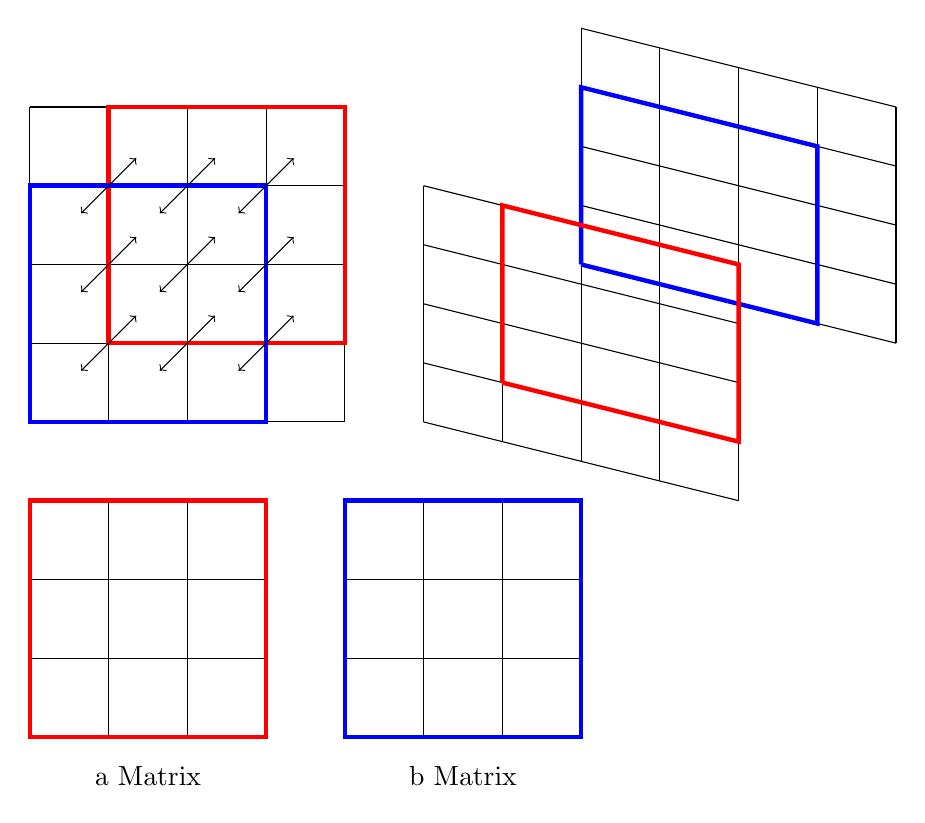
\begin{tikzpicture}

\foreach \x in {0, ..., 4} {
\draw (\x, 0) -- (\x, 4);
\draw (0, \x) -- (4, \x);

\draw (\x + 5, 0 - \x * 0.25) -- (\x + 5, 3 - \x * 0.25);
\draw (\x + 7, 2 - \x * 0.25) -- (\x + 7, 5 - \x * 0.25);

\draw (5, \x * 0.75) -- (9, \x * 0.75 - 1);
\draw (7, 2 + \x * 0.75) -- (11, \x * 0.75 + 1);
}

\draw [ultra thick, blue] (7, 2) -- (7, 4.25) -- (10, 3.5) -- (10, 1.25) -- (7, 2);

\draw [ultra thick, red] (6, 0.5) -- (6, 2.75) -- (9, 2) -- (9, -0.25) -- (6, 0.5);


\draw [ultra thick, red] (1, 1) rectangle (4, 4);
\draw [ultra thick, blue] (0, 0) rectangle (3, 3);

\foreach \x in {0, ..., 3} {
\draw (\x, -4) -- (\x, -1);
\draw (0, \x - 4) -- (3, \x - 4);

\draw (\x + 4, -4) -- (\x + 4, - 1);
\draw (4, \x - 4) -- (7, \x - 4);
}

\draw [ultra thick, red] (0, -4) rectangle (3, -1);
\draw [ultra thick, blue] (4, -4) rectangle (7, -1);

\node at (1.5,-4.5) {a Matrix};
\node at (5.5,-4.5) {b Matrix};

\foreach \x in {0, ..., 2} {
\foreach \y in {0, ..., 2} {
\draw [<->] (0.65 + \x, 0.65 + \y) -> (1.35 + \x, 1.35 + \y);
}
}

\end{tikzpicture}
\caption{a, b from a single 2-D matrix}
\label{ij Creation}
\end{figure}

\subsection{Kernel Convolution}

GLCM works in local kernels, hence we need to partition it somehow. 

It should iterate through all available windows, however, it's time consuming to do the following:

\begin{enumerate}
\item{Split data to sliding windows}
\item{Operate on each window}
\item{Merge all data together}
\end{enumerate}

Hence, we would want to retain the original data as much as possible while mimicking that concept.

\subsubsection{Example}

Let's say we wanted just the sum of all 3x3 kernel windows on $i$ or $j$.

For each 3x3 window, we calculate the following
$$\sum i$$

\begin{figure}[H]
\centering
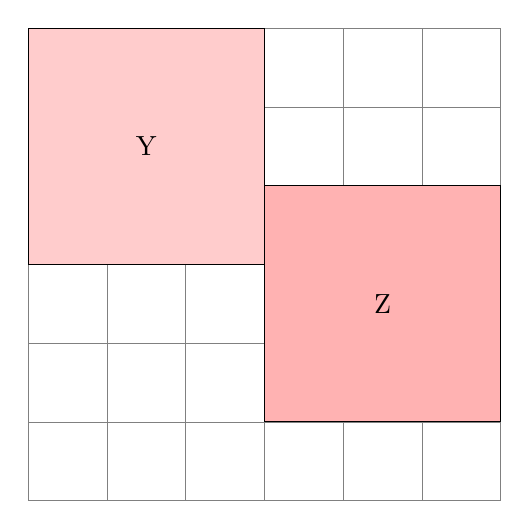
\begin{tikzpicture}
\draw[step=1cm,gray,very thin] (0,0) grid (6,6);
\filldraw[red!20!white, draw=black] (0,6) rectangle (3,3);
\filldraw[red!30!white, draw=black] (3,4) rectangle (6,1);
\node at (1.5, 4.5) {Y};
\node at (4.5, 2.5) {Z};
\end{tikzpicture}
\caption{Y and Z Represents possible 3x3 windows}
\label{Convolution Window Summation}
\end{figure}

This can be solved using a convolution library.

\begin{figure}[H]
\centering
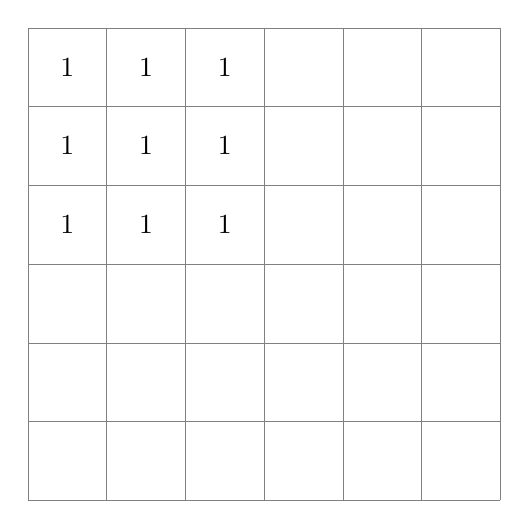
\begin{tikzpicture}
\draw[step=1cm,gray,very thin] (0,0) grid (6,6);
\foreach \x in {0, ..., 2}
\foreach \y in {0, ..., 2}
\node (\x\y) at (0.5+\x,3.5+\y) {1};
\end{tikzpicture}
\caption{A 3x3 Ones Convolution Kernel}
\label{Convolution Window Kernel}
\end{figure}

Using this 3x3 kernel, we can do a sliding window summation for all \textbf{valid} cells.

\begin{figure}[H]
\centering
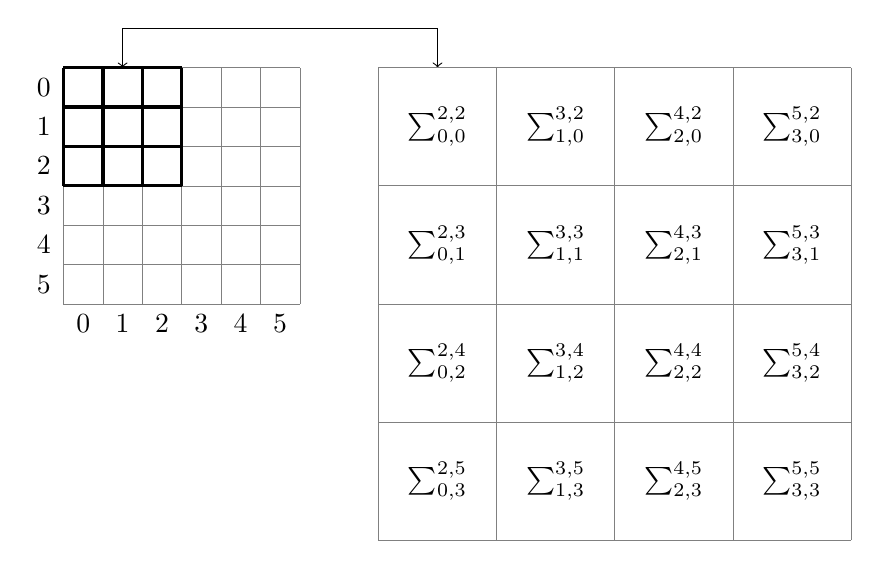
\begin{tikzpicture}

\draw[step=0.5cm,gray,ultra thin] (-4,2.999) grid (-1,6);
\draw[step=0.5cm,black,very thick] (-4,4.499) grid (-2.5,6);

\draw[<->] (-3.25,6) -- (-3.25,6.5) -- (0.75, 6.5) -- (0.75, 6);

\foreach \x in {0, ..., 5} {
	\pgfmathtruncatemacro{\xn}{5-\x}
	\node at (-4.25, \x * 0.5 + 3.25) {\xn};
	\node at (\x * 0.5 - 3.75, 2.75) {\x};
}

\draw[step=1.5cm,gray,very thin] (0,0) grid (6,6);
\foreach \x in {0, ..., 3}{
\foreach \y in {0, ..., 3}{
\pgfmathtruncatemacro{\xn}{\x + 2}
\pgfmathtruncatemacro{\yi}{3 - \y}
\pgfmathtruncatemacro{\yn}{5 - \y}
\node at (\x * 1.5 + 0.75, \y * 1.5 + 0.75) {$\sum_{\x,\yi}^{\xn,\yn}$};
}
}
\end{tikzpicture}

\caption{3x3 Convolution Summation}
\label{Convolution Window Result}
\end{figure}

A more detailed example utilizing this concept can be found in the section \textbf{Contrast} below.

\newpage
\section{Contrast}

Contrast is defined as such

$$\sum_{i=i_0,j=j_0}^{i=i,j=j}(i - j)^2*n_{i,j}$$

Let's say we have the following image data.
We will do a 1-step diagonal GLCM.

\begin{figure}[H]
\centering
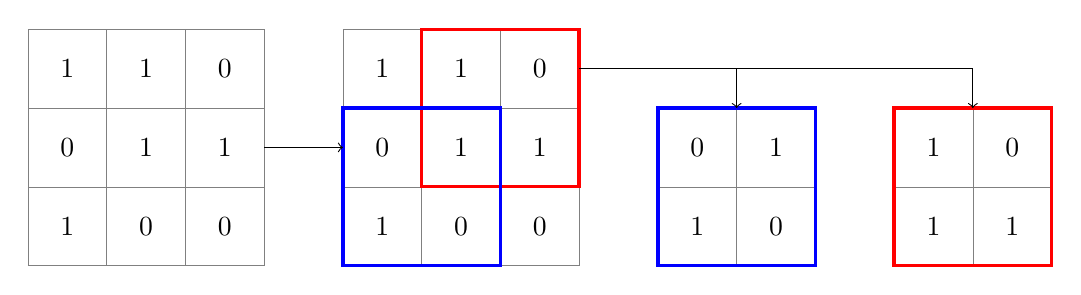
\begin{tikzpicture}
\draw[step=1cm,gray,very thin] (-4,0) grid (-1,3);
\node at (-3.5, 0.5) {1};
\node at (-3.5, 1.5) {0};
\node at (-3.5, 2.5) {1};
\node at (-2.5, 0.5) {0};
\node at (-2.5, 1.5) {1};
\node at (-2.5, 2.5) {1};
\node at (-1.5, 0.5) {0};
\node at (-1.5, 1.5) {1};
\node at (-1.5, 2.5) {0};

\draw[step=1cm,gray,very thin] (0,0) grid (3,3);
\draw[red, very thick] (1,1) rectangle (3,3);
\draw[blue, very thick] (0,0) rectangle (2,2);
\node at (0.5, 0.5) {1};
\node at (0.5, 1.5) {0};
\node at (0.5, 2.5) {1};
\node at (1.5, 0.5) {0};
\node at (1.5, 1.5) {1};
\node at (1.5, 2.5) {1};
\node at (2.5, 0.5) {0};
\node at (2.5, 1.5) {1};
\node at (2.5, 2.5) {0};

\draw[step=1cm,gray,very thin] (4,0) grid (6,2);
\draw[blue, very thick] (4,0) rectangle (6,2);
\node at (4.5, 0.5) {1};
\node at (4.5, 1.5) {0};
\node at (5.5, 0.5) {0};
\node at (5.5, 1.5) {1};

\draw[step=1cm,gray,very thin] (7,0) grid (9,2);
\draw[red, very thick] (7,0) rectangle (9,2);
\node at (7.5, 0.5) {1};
\node at (7.5, 1.5) {1};
\node at (8.5, 0.5) {1};
\node at (8.5, 1.5) {0};

\draw [->] (-1,1.5) -> (0, 1.5);
\draw (3,2.5) -> (8,2.5);

\draw [->] (5,2.5) -> (5,2);
\draw [->] (8,2.5) -> (8,2);

\end{tikzpicture}
\caption{Example GLCM Pair Making}
\label{Example GLCM Pair Making}
\end{figure}

If we were to calculate the GLCM, it'll look something like this

\begin{center}
\begin{tabular}{ |c|c|c| } 
 \hline   & 0 & 1 \\ 
 \hline 0 & 0 & 2 \\ 
 \hline 1 & 1 & 1 \\ 
 \hline
\end{tabular}
\end{center} 

\begin{align*}
\sum(i - j)^2*n
&= (0 - 1) ^ 2 * 2 + (1 - 0) ^ 2 + (1 - 1) ^ 2\\
&= (0 - 1) ^ 2 + (0 - 1) ^ 2 + (1 - 0) ^ 2 + (1 - 1) ^ 2\\
&= 3
\end{align*}

Notice how we expanded $n$, so we can vectorize it.

Let's say we don't generate the GLCM, instead we have the data as so, right after the \textbf{pair making}.

\begin{figure}[H]
\centering
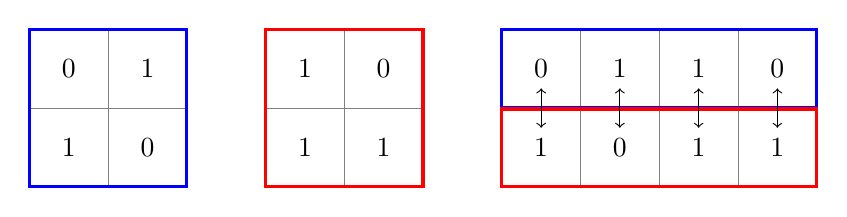
\begin{tikzpicture}

\draw[step=1cm,gray,very thin] (0,0) grid (2,2);
\draw[blue, very thick] (0,0) rectangle (2,2);
\node at (0.5, 0.5) {1};
\node at (0.5, 1.5) {0};
\node at (1.5, 0.5) {0};
\node at (1.5, 1.5) {1};

\draw[step=1cm,gray,very thin] (3,0) grid (5,2);
\draw[red, very thick] (3,0) rectangle (5,2);
\node at (3.5, 0.5) {1};
\node at (3.5, 1.5) {1};
\node at (4.5, 0.5) {1};
\node at (4.5, 1.5) {0};

\draw[step=1cm,gray,very thin] (6,1) grid (10,2);
\draw[blue, very thick] (6,1.01) rectangle (10,2);
\node at (6.5, 1.5) {0};
\node at (7.5, 1.5) {1};
\node at (8.5, 1.5) {1};
\node at (9.5, 1.5) {0};

\draw[step=1cm,gray,very thin] (6,0) grid (10,1);
\draw[red, very thick] (6,0) rectangle (10,0.99);
\node at (6.5, 0.5) {1};
\node at (7.5, 0.5) {0};
\node at (8.5, 0.5) {1};
\node at (9.5, 0.5) {1};

\foreach \xa in {0, ..., 3} {
	\draw [<->] (6.5 + \xa, 0.75) -- (6.5 + \xa, 1.25);
}

\end{tikzpicture}
\caption{Flattening for Vectorization}
\label{Flattening for Vectorization}
\end{figure}

\begin{align*}
\sum(i - j)^2*n
&= (0 - 1) ^ 2 + (1 - 0) ^ 2 + (1 - 0) ^ 2 + (1 - 1) ^ 2\\
&= 3
\end{align*}

As you can see, we managed to avoid GLCM entirely because of the 
linear property of a summation.

We will use the same idea for \textbf{Correlation} below.

\newpage
\section{Correlation}

Correlation is defined as such

$$
\sum_{i=i_0,j=j_0}^{i=i,j=j}
\frac{(i * j) * n_{i,j} - (\mu_x - \mu_y)}
{\sigma_x * \sigma_y}
$$

Where $\mu_x,\mu_y$ are defined as the mean of all $i$ and $j$ values respectively.

$\sigma_x,\sigma_y$ are defined as the standard deviation of $i$ and $j$ values respectively.

To make this formula simpler and relevant for our \textbf{Making Pairs} method, we reword it as such

$$
\sum_{w=w_0}^{w=w} \sum_{a=a_0,b=b_0}^{a=a,b=b}
\frac{(a * b) - (\mu_a - \mu_b)}
{\sigma_a * \sigma_b}
$$

In simpler terms

\begin{verbatim}
for a and b in each window pair:
	(
		sum all (a * b) cells
		minus mean of a
		plus mean of b # Note the sign!
	)	
	all divided by
	(
		standard deviation of a 
		multiplied by standard deviation of b
	)
\end{verbatim}

Notice how we need to calculate the mean and standard deviation
\textbf{within} each window pair. This raises a problem where
we need to \textbf{Convolute} within the \textbf{Window Convolution}. 

This is referred to as the \textit{Inner Convolution}.

\begin{figure}[H]
\centering
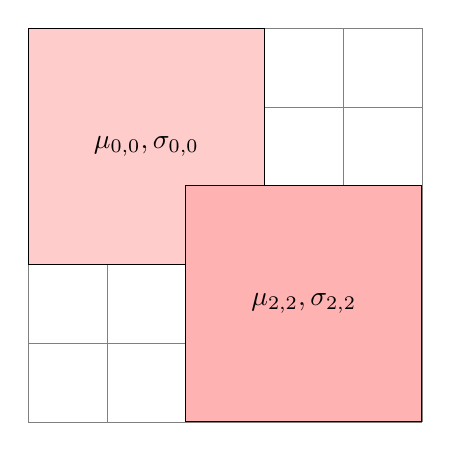
\begin{tikzpicture}
\draw[step=1cm,gray,very thin] (0,0) grid (5,5);
\filldraw[red!20!white, draw=black] (0,5) rectangle (3,2);
\filldraw[red!30!white, draw=black] (2,3) rectangle (5,0);
\node at (1.5, 3.5) {$\mu_{0,0}, \sigma_{0,0}$};
\node at (3.5, 1.5) {$\mu_{2,2}, \sigma_{2,2}$};
\end{tikzpicture}
\caption{Correlation Inner Convolution 3x3}
\label{Correlation Inner Convolution 3x3}
\end{figure}

\subsection{Inner Convolution Mean}

Let's deal with $\mu$, the mean first.

\begin{figure}[H]
\centering
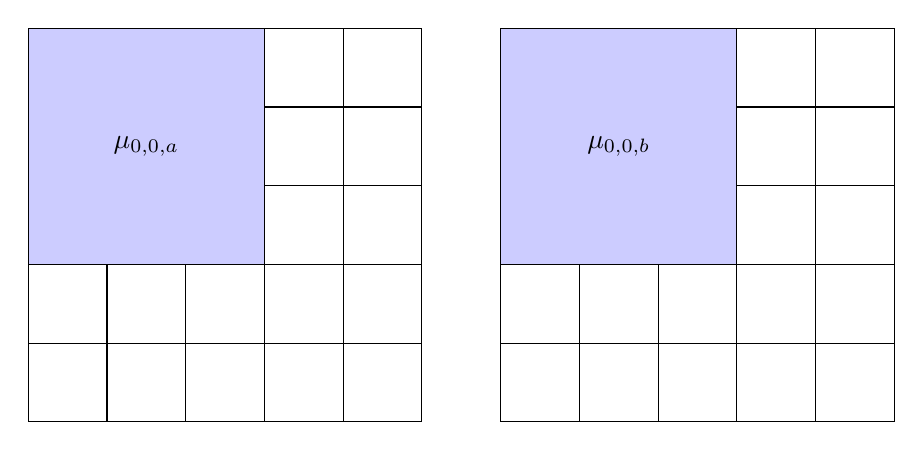
\begin{tikzpicture}
\foreach \xa in {0, ..., 5} {
	\draw[black] (\xa, 0) -- (\xa, 5);
	\draw[black] (0, \xa) -- (5, \xa);
	
	\draw[black] (\xa + 6, 0) -- (\xa + 6, 5);
	\draw[black] (6, \xa) -- (11, \xa);
}

\filldraw[blue!20!white, draw=black] (6,5) rectangle (9,2);
\filldraw[blue!20!white, draw=black] (0,5) rectangle (3,2);
\node at (1.5, 3.5) {$\mu_{0,0,a}$};
\node at (7.5, 3.5) {$\mu_{0,0,b}$};
\end{tikzpicture}
\caption{Correlation Inner Convolution Mean}
\label{Correlation Inner Convolution Mean}
\end{figure}

In order to integrate this with a convolution, we just need to create a \textbf{ones kernel} then divide by the size or \textbf{$1/size$ kernel} and convolute that window across the data.

\subsection{Inner Convolution Standard Deviation}

We'll look at $\sigma$, which causes a bit of an issue.

The standard deviation function cannot be attached to the convolution \textbf{directly}. However, thankfully, we have an alternative formula.

\textit{Note: We only depict a here}

\begin{align*}
Var    &= E(A^2) - E(A)^2 \\
\sigma &= \sqrt{E(A^2) - E(A)^2}
\end{align*}

\begin{figure}[H]
\centering
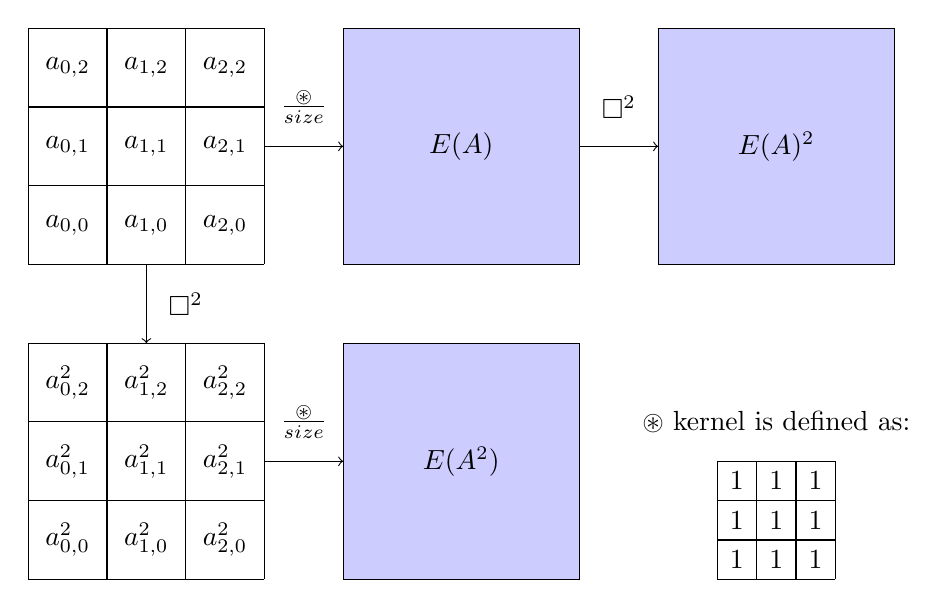
\begin{tikzpicture}
\foreach \xa in {0, ..., 3} {
	\draw[black] (\xa, 0) -- (\xa, 3);
	\draw[black] (0, \xa) -- (3, \xa);
	
	\filldraw[blue!20!white, draw=black] (4,3) rectangle (7,0);
	\filldraw[blue!20!white, draw=black] (4,7) rectangle (7,4);
	\filldraw[blue!20!white, draw=black] (8,7) rectangle (11,4);
	
	\draw[black] (\xa, 4) -- (\xa, 7);
	\draw[black] (0, \xa + 4) -- (3, \xa + 4);
	
	\draw[black] (\xa * 0.5 + 8.75, 0) -- (\xa * 0.5 + 8.75, 1.5);
	\draw[black] (8.75, \xa * 0.5) -- (10.25, \xa * 0.5);
}

\foreach \xa in {2, ..., 0} {
	\foreach \ya in {0, ..., 2} {
		\node at (\xa + 0.5, \ya + 4.5) {$a_{\xa, \ya}$};
		\node at (\xa + 0.5, \ya + 0.5) {$a_{\xa, \ya}^2$};
		\node at (\xa * 0.5 + 9, \ya * 0.5 + 0.25) {$1$};
	}
}

\node at (5.5, 5.5) {$E(A)$};
\node at (5.5, 1.5) {$E(A^2)$};
\node at (9.5, 5.5) {$E(A)^2$};
\draw [->] (1.5, 4) -- (1.5, 3);
\draw [->] (3, 1.5) -- (4, 1.5);
\draw [->] (3, 5.5) -- (4, 5.5);
\draw [->] (7, 5.5) -- (8, 5.5);

\node at (2, 3.5) {$\square^2$};
\node at (3.5, 2) {$\frac{\circledast}{size}$};
\node at (3.5, 6) {$\frac{\circledast}{size}$};
\node at (7.5, 6) {$\square^2$};
\node at (9.5, 2) {$\circledast$ kernel is defined as:};

\end{tikzpicture}
\caption{Correlation Inner Convolution Standard Deviation}
\label{Correlation Inner Convolution Standard Deviation}
\end{figure}

Using this flow-chart, we can get our standard deviation locally for each kernel.

The rest of the steps are similar to \textbf{Contrast}, so I won't repeat it. The following shows a summary on how it's done in python.

\begin{figure}[H]
\begin{python}
kernel = np.ones(shape=[radius * 2 + 1, radius * 2 + 1, 1])

conv_ab = fftconvolve(a * b, kernel, mode='valid')

# E(A) 
conv_a = fftconvolve(ai, kernel, mode='valid')
conv_ae = conv_a / kernel.size

# E(A^2)
conv_a2 = fftconvolve(a ** 2, kernel, mode='valid')
conv_ae2 = conv_i2 / kernel.size

# E(A)^2
conv_ae_2 = conv_ae ** 2

# Stdev(A)
conv_stda = np.sqrt(np.abs(conv_ae2 - conv_ae_2))

cor = (conv_ab - (conv_ae - conv_be)) / conv_stda * conv_stdb
\end{python}

\caption{Correlation Algorithm Summary. Self-explanatory variables are removed.}
\label{Correlation Algorithm Summary}
\end{figure}

\newpage
\section{Entropy}

This is one of the statistics that is not possible to vectorize efficiently.

Entropy is defined as such

$$\sum_{i=i_0,j=j_0}^{i=i,j=j} n^2$$

In other words, every occurrence is squared, then summed. Due to the squaring on the occurrences, we cannot simplify it for convolution vectorization.

Note that we'll use the GLCM convention $i, j$ here instead of $a, b$.

\begin{figure}[H]
\centering
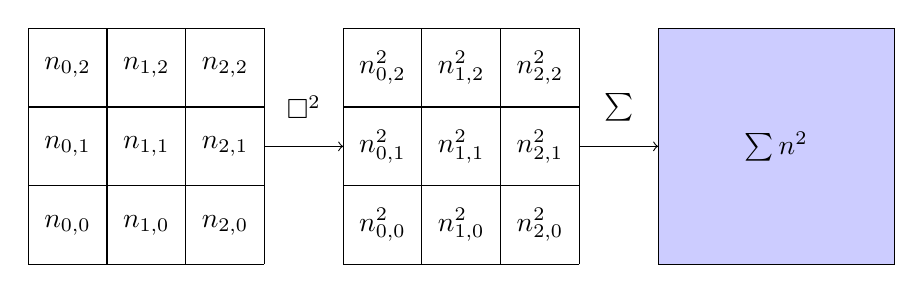
\begin{tikzpicture}
\foreach \xa in {0, ..., 3} {
	\draw[black] (\xa, 0) -- (\xa, 3);
	\draw[black] (0, \xa) -- (3, \xa);
	
	\draw[black] (\xa+4, 0) -- (\xa+4, 3);
	\draw[black] (4, \xa) -- (7, \xa);

	\filldraw[blue!20!white, draw=black] (8,3) rectangle (11,0);
	
}

\foreach \xa in {2, ..., 0} {
	\foreach \ya in {0, ..., 2} {
		\node at (\xa + 0.5, \ya + 0.5) {$n_{\xa, \ya}$};
		\node at (\xa + 4.5, \ya + 0.5) {$n_{\xa, \ya}^2$};
	}
}

\node at (9.5, 1.5) {$\sum n^2$};
\draw [->] (3, 1.5) -- (4, 1.5);
\draw [->] (7, 1.5) -- (8, 1.5);

\node at (3.5, 2) {$\square^2$};
\node at (7.5, 2) {$\sum$};

\end{tikzpicture}
\caption{Entropy Calculation}
\label{Entropy Calculation}
\end{figure}

\subsection{Brute Force Approach}

The current approach is simple

\begin{enumerate}
\item{Multiply one by $256$ and add both together}
\item{Partition summed data with an $n*n$ sliding window}
\item{For each window, we calculate local entropy}
\end{enumerate}

\subsubsection{NumPy Unique and Bin Count}

There's an issue with \verb+np.unique+ and \verb+np.bin_count+, where it doesn't operate on multiple axes correctly.

Hence we require both $i, j$ to be represented as a singular value.

\begin{align*}
(i, j) &\in \mathbb{Z}\\
max(i, j) &= (255, 255)\\
f(i, j)   &= i * 256 + j\\
\end{align*}

For all $(i, j)$ pairs, there's a unique $f(i, j)$ value.

Hence, we can call \verb+np.unique+ or \verb+np.bin_count+ on a the single dimension.

\subsubsection{Performance of NumPy Unique and Bin Count}

Tested it out with a small 200 x 200 image, \verb+np.bin_count+ seems to be the faster alternative.

\subsubsection{Sliding Window}

Instead of using \textbf{Convolution} as per the previous statistics, we have to use a sliding window as \verb+np.bin_count+ can't be vectorized.

\subsubsection{Entropy Calculation}

For each local sliding window, we can simply call \verb+np.bin_count+ on it then square each occurrence, then sum it.

\begin{python}
entropy = np.sum(np.bincount(w) ** 2)
\end{python}

\subsection{COO Sparse Matrix Approach}

This is an alternative approach, where it's significantly slower, however it may be improved with low-level tweaking.

\textbf{COO} is a Co-ordinate based sparse matrix.

A \textbf{Sparse Matrix} is any matrix that is expected to have large amounts of \textit{null values}, like 0.

By making $i, j$ coordinates and feeding it into \verb+scipy.sparse.coo_matrix+, it implicitly sums up occurrences. Hence, we can extract them as a \verb+np.ndarray+ and square sum it.

However, because it doesn't integrate well with multiple channels, discussed later, it is slower than \textbf{Brute Force}.

\begin{python}
    
coo_r = coo_matrix((cd, (ca[..., 0], cb[..., 0])),
                    shape=(MAX_RGB, MAX_RGB))
                    .tocsr(copy=False).power(2).sum()
coo_g = coo_matrix((cd, (ca[..., 1], cb[..., 1])),
                    shape=(MAX_RGB, MAX_RGB))
                    .tocsr(copy=False).power(2).sum()
coo_b = coo_matrix((cd, (ca[..., 2], cb[..., 2])),
                    shape=(MAX_RGB, MAX_RGB))
                    .tocsr(copy=False).power(2).sum()
    
\end{python}

Notice how each channel must run their own \verb+coo_matrix+, I speculate that its performance decreases here.

\subsection{Multi Processing}

In the library, I included an option to use multiple processors to loop on separate threads.

This is possible because it's a for-loop, this makes the entropy looping much faster.

\section{Multiple Channels}

One major consideration for the above algorithms is that it must work with multiple channels as we're looking for the following 

\begin{center}
\begin{tabular}{ |c|c|c|c| } 
 \hline   & Con  & Cor  & Ent  \\ 
 \hline R & ConR & CorR & EntR \\
 \hline G & ConG & CorG & EntG \\
 \hline B & ConB & CorB & EntB \\
 \hline
\end{tabular}
\end{center} 

Making a poor non-vectorized algorithm will result in heavy delays as they are processed linearly.

As most operations work with \verb+np.ndarray+, most of it works fine with additional axes.

\subsection{Channel Dimension}

Those unfamiliar on how my data is original represented may find this useful.

An example of my original data would be \verb+[3, 4, 3]+.

This means, 3 rows, 4 columns, 3 channels.
If they were RGB channels, then it'll look like the following figures.

\begin{figure}[H]
\centering
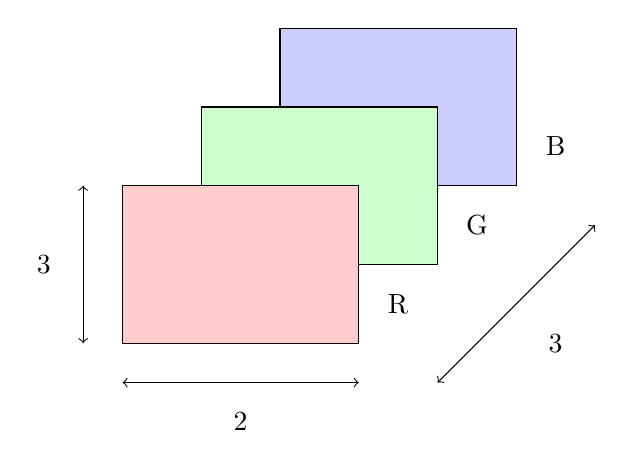
\begin{tikzpicture}

\filldraw[blue!20!white, draw=black]  (2,5) rectangle (5,3);
\filldraw[green!20!white, draw=black] (1,4) rectangle (4,2);
\filldraw[red!20!white, draw=black]   (0,3) rectangle (3,1);

\node at (3.5, 1.5) {R};
\node at (4.5, 2.5) {G};
\node at (5.5, 3.5) {B};

\draw [<->] (0, 0.5) -- (3, 0.5);
\draw [<->] (-0.5, 1) -- (-0.5, 3);
\draw [<->] (4, 0.5) -- (6, 2.5);

\node at (1.5, 0) {2};
\node at (-1, 2)  {3};
\node at (5.5, 1) {3};

\end{tikzpicture}
\caption{Channel Dimension Example 1}
\label{Channel Dimension Example 1}
\end{figure}

\begin{figure}[H]
\centering
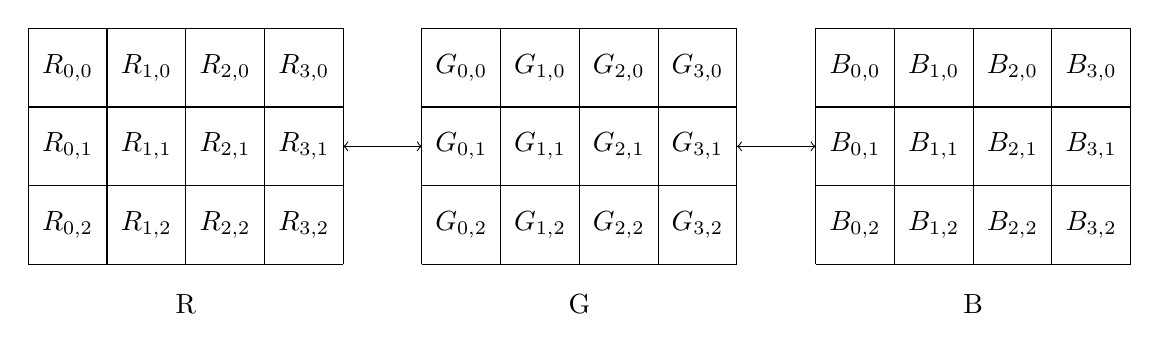
\begin{tikzpicture}
\foreach \xa in {0, ..., 4} {
	\draw[black] (\xa, 0) -- (\xa, 3);
	\draw[black] (\xa+5, 0) -- (\xa+5, 3);
	\draw[black] (\xa+10, 0) -- (\xa+10, 3);
}

\foreach \xa in {0, ..., 3} {
	\draw[black] (0, \xa) -- (4, \xa);
	\draw[black] (5, \xa) -- (9, \xa);
	\draw[black] (10, \xa) -- (14, \xa);
}

\foreach \xa in {0, ..., 3} {
	\foreach \ya in {0, ..., 2} {
		\pgfmathtruncatemacro{\yn}{2 - \ya}
		\node at (\xa + 0.5, \ya + 0.5) {$R_{\xa, \yn}$};
		\node at (\xa + 5.5, \ya + 0.5) {$G_{\xa, \yn}$};
		\node at (\xa + 10.5, \ya + 0.5) {$B_{\xa, \yn}$};
	}
}

\draw [<->] (4, 1.5) -- (5, 1.5);
\draw [<->] (9, 1.5) -- (10, 1.5);

\node at (2, -0.5) {R};
\node at (7, -0.5) {G};
\node at (12, -0.5) {B};

\end{tikzpicture}
\caption{Channel Dimension Example 2 }
\label{Channel Dimension Example 2}
\end{figure}

The last dimensions is always the \textit{Channel Dimension}.

Hence if I would want to call operations on separate channels, I'd just have to specify to split on the last axis.





\section{Other Channels}

As of now GLCM works only with RGB, but can be adapted to other channels with tweaking.

\begin{itemize}
\item{Entropy assumes RGB, hence it may need to multiply by other values other than $256$ if changed}
\item{Entropy assumes integer inputs, \verb+np.bin_count+ only works with integers, \verb+np.unique+ can be used but with a decrease in performance}
\end{itemize}

\newpage
\chapter{Code Annex}

\section{Contrast}

\begin{python}
ar = (rgb_a - rgb_b) ** 2
     return fftconvolve(ar,
                        np.ones(shape=[radius * 2 + 1,
                                       radius * 2 + 1, 1]),
                        mode='valid')
\end{python}

\section{Correlation}

\begin{python}
kernel = np.ones(shape=[radius * 2 + 1, radius * 2 + 1, 1])

conv_ab = fftconvolve(rgb_a * rgb_b, kernel, mode='valid')

conv_a = fftconvolve(rgb_a, kernel, mode='valid')
conv_b = fftconvolve(rgb_b, kernel, mode='valid')

# E(A) & E(B)
conv_ae = conv_a / kernel.size
conv_be = conv_b / kernel.size

conv_a2 = fftconvolve(rgb_a ** 2, kernel, mode='valid')
conv_b2 = fftconvolve(rgb_b ** 2, kernel, mode='valid')

# E(A^2) & E(B^2)
conv_ae2 = conv_a2 / kernel.size
conv_be2 = conv_b2 / kernel.size

# E(A)^2 & E(B)^2
conv_ae_2 = conv_ae ** 2
conv_be_2 = conv_be ** 2

conv_stda = np.sqrt(np.abs(conv_ae2 - conv_ae_2))
conv_stdb = np.sqrt(np.abs(conv_be2 - conv_be_2))

with np.errstate(divide='ignore', invalid='ignore'):
    cor = (conv_ab - (conv_ae - conv_be)) / conv_stda * conv_stdb
    return np.nan_to_num(cor, copy=False, nan=0, neginf=-1, posinf=1)
\end{python}


\section{Entropy}

\begin{python}
rgb_a = rgb_a.astype(np.uint16)
rgb_b = rgb_b.astype(np.uint16)

cells = view_as_windows(self.init(rgb_a * (MAX_RGB + 1) + rgb_b).data,
                        [radius * 2 + 1, radius * 2 + 1,3],
                        step=1).squeeze()

out = np.zeros((rgb_a.shape[0] - radius * 2,
                rgb_a.shape[1] - radius * 2,
                3))  # RGB count

for row, _ in enumerate(cells):
    for col, cell in enumerate(_):
        c = cell.reshape([-1, cell.shape[-1]])
        entropy = np.asarray([np.sum(np.bincount(g) ** 2)
                              for g in c.swapaxes(0, 1)])
        out[row, col, :] = entropy
return out
\end{python}

\section{Entropy Multiprocessing}

\begin{python}
p = Pool(procs) if procs else Pool()

for i, _ in enumerate(p.imap_unordered(self._get_glcm_entropy_mp_loop, cells)):
    out[i, :, :] = _

return out
\end{python}

\section{Entropy COO (Deprecated)}

Some functions may be deprecated.

\begin{python}
w_a = self.init(rgb_a).slide_xy(by=radius * 2 + 1, stride=1)
w_b = self.init(rgb_b).slide_xy(by=radius * 2 + 1, stride=1)

out = np.zeros((rgb_a.shape[0] - radius * 2,
                rgb_a.shape[1] - radius * 2,
                3))  # RGB * Channel count

for col, (_a, _b) in enumerate(zip(w_a, w_b)):
    if verbose: print(f"GLCM Entropy: {col} / {len(w_a)}")
    for row, (ca, cb) in enumerate(zip(_a, _b)):
        # We flatten the x and y axis first.
        ca = ca.data.reshape([-1, ca.shape[-1]])
        cb = cb.data.reshape([-1, cb.shape[-1]])
        cd = np.ones(ca.shape[0])

        coo_r = coo_matrix((cd, (ca[..., 0], cb[..., 0])),
                            shape=(MAX_RGB, MAX_RGB))
                            .tocsr(copy=False).power(2).sum()
        coo_g = coo_matrix((cd, (ca[..., 1], cb[..., 1]))
                            shape=(MAX_RGB, MAX_RGB))
                            .tocsr(copy=False).power(2).sum()
        coo_b = coo_matrix((cd, (ca[..., 2], cb[..., 2]))
                            shape=(MAX_RGB, MAX_RGB))
                            .tocsr(copy=False).power(2).sum()

        out[row, col, :] = [coo_r, coo_g, coo_b]

return out
\end{python}
\end{document}

